\chapter{Introducción}\label{cha:introduccion}

\section{Presentación del Documento}

El presente informe describe el proyecto de desarrollo Gestión de repositorios semánticos compatible con el estándar \acrshort{oaipmh}, un aplicativo que pretende extender a \acrshort{labman}, el \acrlong{dms} de los grupos de Internet y Telecomunicaciones de DeustoTech, detallando tanto los objetivos que se pretenden alcanzar con el proyecto, como las fases, actividades y recursos necesarios para llevarlo a cabo.

El contenido de este documento se estructura en torno a los siguientes productos:

\begin{itemize}
	\item \textbf{Introducción a \acrshort{labman}:}

	Breve introducción a \acrshort{labman} y a las tecnologías y de las tecnologías que lo conforman, incluyendo un breve estudio de las ventajas e inconvenientes de las mismas, finalizando con una conclusión sobre el uso de las mismas.

	\item \textbf{Definición de proyecto:}
		
	Establecimiento del objetivo fundamental del proyecto, especificando cuáles son los aspectos funcionales que lo comprenden y cuáles son los que quedan excluidos.
	
	\item \textbf{Producto final:}
		
	Especificación de la solución elegida que va a construir el proyecto en cuestión.
	
	\item \textbf{Descripción de la realización:}

	Realización y definición de las diferentes actividades cuyo desarrollo va a permitir la realización y consecución del objetivo del proyecto.

	\item \textbf{Organización:}
	
	Definición del equipo de trabajo que desarrollará el proyecto, así como su estructura organizativa, sistema de gestión y seguimiento del trabajo.

	\item \textbf{Condiciones de ejecución:}

	Definición del entorno de trabajo, de los criterios sobre los que se van a realizar las sucesivas recepciones, así como el tratamiento que se va a establecer para aquellos casos que puedan ser considerados como modificaciones o mejoras en el planteamiento inicial del proyecto.

	\item \textbf{Planificación:}
	
	Estimación de cargas y duración de las diferentes actividades del proyecto, así como su asignación a los diferentes miembros del equipo y su planificación en el tiempo.

	\item \textbf{Valoración económica:}
	
	Determinación del valor correspondiente a este proyecto, de los hitos de facturación y de la forma de pago.

	\item \textbf{Desarrollo del proyecto:}
	
	Especificación de Requisitos del Sistema Especificación del Diseño Consideraciones sobre la Implementación Plan de Pruebas Manual de Usuario Incidencias del Proyecto.

	\item \textbf{Conclusiones y líneas futuras:}


\end{itemize}

\section{Introducción a LabMan}

Es este apartado se realiza una breve introducción a \acrfull{labman}, el \acrlong{dms} de MoreLab, el grupo de investigación formado por los equipos de Internet y Telecomunicaciones de DeustoTech y en el que se basa este proyecto.

\begin{figure}[!htp]
	\centering
	
\includegraphics[scale=0.15]{fig/morelab-logo}
	\caption{Logo de MORELab}
\end{figure}

Gestionar la información no siempre es una tarea trivial y más aún cuando hay que tratar con los datos que componen varias entidades como pueden ser los proyectos, investigadores, publicaciones, eventos, etc. dentro del ámbito de la investigación. La mayoría de los grupos de investigación utilizan sistemas de gestión de contenido tales como Joomla!\cite{joomla}, WordPress\cite{wordpress} o Drupal\cite{drupal} para exponer sus datos. Sin embargo, para extraer la información de estos \acrshortpl{cms} se requieren herramientas externas para llevar a cabo técnicas de análisis de datos. 
Para hacer uso de estas herramientas normalmente hace falta generar documentos adicionales, tales como \acrshort{csv}, ficheros de texto, entre otros que provocan redundancia de la información, que provoca dificultades a la hora de actualizar los datos y la calidad de los mismos. Esta situación empeora cuando además se disponen de distintas fuentes para la obtención de información, como pueden ser las paginas web personales de los investigadores en los que se muestran sus logros a lo largo de su carrera, la información financiera gestionada por su propio departamento, etc.

Del esfuerzo para gestionar la información grupo de investigación de MoreLab nace {labman}, con el objetivo de gestionar todo este tipo información diferenciadose de otros \acrshort{cms} por apostar por la exposición de los datos como \acrlong{lod}\cite{linkeddata}.

Los datos enlazados\cite{pena_visual_2014}
\section{Introducción a SQL}

Como su propio nombre indica, \acrfull{sql} es un lenguaje de programación, estandarizado por \acrshort{iso}\cite{ISO} y \acrshort{ansi}\cite{ANSI}, diseñado para gestionar la información almacenada en los sistemas de gestión de bases de datos relacionales, como por ejemplo PostgreSQL\cite{PostgreSQL}, MySQL\cite{MySQL}, SQLite\cite{SQLite}, por medio de consultas estructuradas en inglés.

Las consultas representan las operaciones más comunes y esenciales del lenguaje \acrshort{sql} para la recopilación de información dentro de una \acrshort{bd}. Estas consultas se realizan por medio de la sentencia ``SELECT'', que pueden ser complementadas por medio de clausulas para realizar búsquedas específicas. De todas las clausulas disponibles hay que destacar la siguientes:

\begin{itemize}
	\item \textbf{FROM:} Indica de que tabla o tablas de debe extraerse la información.
	\item \textbf{WHERE:} Sirve para delimitar las tuplas o filas de la tablas en las que se realiza la búsqueda. Si las filas no cumplen las condiciones expuestas en esta clausula, serán excluidas del resultado.
	\item \textbf{ORDER BY:} Esta es la única forma para definir el criterio de ordenación los resultados en \acrshort{sql}, sin esta clausula el orden sería aleatorio.
\end{itemize}

\lstinputlisting[language=SQL, frame=single, label={lst:selectsql}, caption=Ejemplo de sentencia SELECT en \acrshort{sql}]{content/code/sql/select-example.sql}

En esta consulta \acrshort{sql} (ver algoritmo \ref{lst:selectsql}) se solicitan todos los nombres y las ciudades de los clientes que residan en Suecia.
\section{Introducción a SPARQL}

\acrshort{sparql}\cite{SPARQL_language} es el acrónimo recursivo del inglés \acrlong{sparql} que hace referencia tanto a el lenguaje estandarizado por la \acrshort{rdf} \acrshort{dawg} de la \acrshort{w3c}\cite{W3C} para consultas a grafos \acrshort{rdf} como para el protocolo de invocación de consultas \acrshort{sparql} remotas.

El lenguaje de consultas \acrshort{sparql} (actualmente en la versión 1.1), permite tanto buscar como manipular grafos \acrshort{rdf} disponibles en la web o bases de datos semánticas almacenados como tripletas, en otras palabras, define un lenguaje equivalente a \acrshort{sql} a excepción de que este se utiliza exclusivamente para bases de datos semánticas.

Al igual que en \acrshort{sql} las consultas en \acrshort{sparql} constituyen las operaciones más comunes y esenciales del lenguaje. Su estructura es es muy similar a la ya vista en el algoritmo \ref{lst:selectsql}, haciendo uso de la misma sentencia ``SELECT''.

\lstinputlisting[language=SQL, otherkeywords={PREFIX}, frame=single, label={lst:selectsparql}, caption=Ejemplo de sentencia SELECT en \acrshort{sparql}]{content/code/sparql/select-example.sparql}

Esta consulta \acrshort{sparql} (ver algoritmo \ref{lst:selectsparql}) añade un nuevo elemento ``PREFIX'' a lo anteriormente visto en \acrshort{sql}, que tiene como función almacenar \acrshortpl{uri} para reducir la longitud de de las mismas a la hora de acceder a sus atributos. La consulta en sí busca en los sujetos ?planttype y los objetos ?name que estén relacionado con el predicativo plant:planttype y devuelve solo sus nombres.
\section{Introducción a OAI-PMH}

\acrfull{oaipmh} (actualmente disponible en su versión 2.0) es un protocolo para la transmisión de metadatos en Internet que surgió del esfuerzo de mejorar y abrir el acceso a archivos de publicaciones electrónicas (e-prints) y en general a un gran rango de materiales digitales que ha despertado el interés de la comunidad de bibliotecarios.\cite{JM_OAI}

\begin{figure}[!htp]
	\centering
	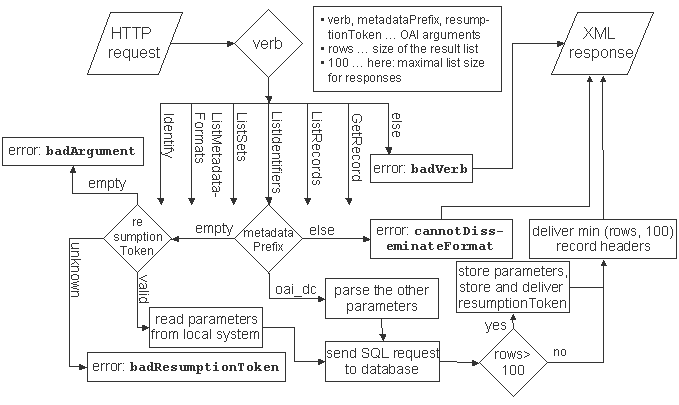
\includegraphics[scale=.15]{fig/oai_flow}
	\caption{Diagrama de flujo del servidor \acrshort{oaipmh}}\label{fig:oaiflow}
\end{figure}

El protocolo \acrshort{oaipmh} se basa en una arquitectura cliente-servidor en la que el cliente realiza las consultas por medio de transacciones \acrshort{http} GET o POST constituidas por un conjunto de opciones del tipo clave=valor. El servidor responde a la petición devolviendo un documento \acrshort{xml} bajo al menos el estandar \acrfull{dc}, según dicta la especificación de la implementación mínima del protocolo \acrshort{oaipmh} para los proveedores de información.\cite{OAIPMH_implementers}

Como se ve en la figura \ref{fig:oaiflow}\cite{oai_implementation} el cliente puede realizar seis peticiones al servidor en función del valor especificado en el `verb' de la consulta, las peticiones pueden ser:

\begin{itemize}
	\item \textbf{Idenfity:} Envía información sobre el servidor, así como el nombre del repositorio, \acrshort{url} base, correo electrónico del administrador del servidor, etc.
	\item \textbf{ListMetadataFormats:} Envía la lista de formatos en los que se encuentran disponibles los metadatos que al menos deben estar disponibles en \acrshort{dc}.
	\item \textbf{ListSets:} Envía una lista con los términos opcionales creados por el servidor para facilitar la recuperación de metadatos selectiva de los registros, posibilitando que un cliente pueda solicitar los registros pertenecientes a una clase en concreto. Estos términos representan una clasificación de los recursos según varias entradas. Los sets pueden estar compuestos por listas simple o formar una jerarquía.
	\item \textbf{ListIdentifiers: } Devuelve la cabecera de hasta un máximo de 100 registros por petición. Los identificadores pueden filtrarse por un rango entre dos fechas de creación o modificación o por los distintos ``sets'' definidos por el servidor.
	\item \textbf{ListRecords: } Realiza la misma tarea que la petición \textit{ListIdentifiers} a excepción de devolver el registro completo con sus metadatos, en lugar de incluir solo la cabecera del recurso. En caso de que la petición resulte una lista de más de 100 recursos, al igual que en la petición \textit{ListIdentifiers}, al final de la lista \acrshort{xml} se devolverá una clave `resumptionToken' que deberá ser utilizada por el cliente para continuar la devolución de los siguientes 100 registros en otra petición \acrshort{http} independiente.
	\item \textbf{GetRecord: } Petición utilizada para devolver un registro en concreto, siendo necesario especificar el identificador del recurso solicitado y el formato bibliográfico en el que se desea que se devuelva.
\end{itemize}

\clearpage

\lstinputlisting[language=XML, frame=single, label={lst:oaipmhgetrecord}, caption=Ejemplo de petición GetRecord de \acrshort{oaipmh}]{content/code/xml/get-record-example.xml}

El \acrshort{xml} generado por el servidor presenta la siguiente estructura para la extracción de los recursos:

\begin{itemize}
	\item \textbf{Información sobre la transacción:} El comienzo del \acrshort{xml} siempre está compuesto por atributos \textit{smlns}, \textit{smlns:xsi} y \textit{xsi:schemaLocation} que sirven para definir ``namespace'' y el esquema de \acrshort{oaipmh} del \acrshort{xml}.

	\item \textbf{La petición en cuestión:} En esta parte del \acrshort{xml} trata la información sobre una de las seis posibles peticiones. En el caso del GetRecords (véase algoritmo \ref{lst:oaipmhgetrecord}) por ejemplo, puede observarse que se compone de un elemento ``record'' y en el se subdivide en:
		\begin{itemize}
			\item Cabecera, en la que se especifica el identificador único, la fecha de creación o última modificación y la lista de ``sets'' a la que pertenece.
			\item Metadatos, la información misma del registro en cuestión compuesto por atributos tales como \textit{dc:title}, \textit{dc:creator}, \textit{dc:subjet}, y en general cualquiera de los atributos definidos en el set de elementos de \acrshort{dc}\cite{DCElements} o el formato bibliográfico que se haya especificado en la consulta.
		\end{itemize}
\end{itemize}
\section{Fortalezas y debilidades de las tecnologías}